\documentclass[a4paper,twoside]{article}

\usepackage{epsfig}
\usepackage{subcaption}
\usepackage{calc}
\usepackage{comment}
\usepackage{amssymb}
\usepackage{amstext}
\usepackage{amsmath}
\usepackage{amsthm}
\usepackage{multicol}
\usepackage{pslatex}
\usepackage{apalike}
\usepackage{xcolor}
\usepackage{multirow}
\usepackage{array}
\usepackage{SCITEPRESS}
\usepackage{graphicx} % Please add other packages that you may need BEFORE the SCITEPRESS.sty package.

\newcommand{\head}[1]{\textbf{#1}}
\newcolumntype{C}[1]{>{\centering\arraybackslash}p{#1}}


\begin{document}

\title{A Case Study on Performance Optimization Techniques in Java Programming}

\author{\authorname{Ciprian Khlud\sup{1}\orcidAuthor{0000-0001-6211-3199}
  and Cristian Fr\u asinaru\sup{1}\orcidAuthor{0000-0002-5246-7396}}
\affiliation{\sup{1}"Alexandru Ioan Cuza University", Ia\c si, Romania}
\email{ciprian.mustiata@gmail.com, acf@info.uaic.ro}
}

\keywords{Java, Runtime performance, Memory usage, Garbage collection, Sequence analysis, SAM/BAM files}

\abstract{
Choosing the right programming platform for processor or memory intensive applications is a subject that is debated in all types of contexts.
%When analyzing the performance of a specific platform, equally important is the usage of appropriate language specific constructions and programming interfaces (APIs).
In this paper we investigate how a state-of-the art implementation, part of a multi-threaded framework for sequence analysis (elPrep)
could benefit from various optimization techniques dedicated to improving the runtime performance of Java applications.
%ElPrep is an established tool for processing SAM and BAM files in sequencing pipelines.
%In order to migrate from its original implementation to a different software platform, more suitable for memory intensive tasks,
%the authors have re-implemented elPrep in Java, Go and C++ and benchmarked their performance.
%Overall, the Go implementation won by a good margin, considering a metric that involved both the RAM usage and the runtime performance.
We show that, without changing the semantics of the algorithm, by using appropriate programming techniques we are able to significantly improve the behavior of the Java implementation to a point that may even alter the conclusions of the original study.
We also show that, by changing the manner in which data is represented, to better fit the particulars of the Java memory management, we are able to improve the original scoring (based on computing time and memory consumption) to around one order of magnitude better on the most expensive component (read/write).
}

\onecolumn \maketitle \normalsize \setcounter{footnote}{0} \vfill

\section{\uppercase{Introduction}}
\label{intro}

In the field of bioinformatics, DNA sequence analysis \cite{doring:2008} generally consists of processing large amounts of data and performing
various operations on it,
such as sequence alignment, variant detection, searches against biological databases, etc.
A large variety of software tools exist for these operations, most of them having specific uses cases but with a common
denominator regarding the fact they need to perform processor and memory intensive tasks: I/O operations on large file,
compression/decompression, text processing, etc.

Choosing a programming platform that offers all the required instruments to handle the specific challenges in
bioinformatics is important,
as pointed out in a recent study dedicated to migrating an existing Common Lisp application, called elPrep, 
to another platform with better support for memory management and concurrency~\cite{costanza:2019}.
ElPrep~\cite{herzeel:2019} is a multi-threaded tool for preparing sequence alignment/map files (SAM/BAM)
for variant calling in DNA sequencing pipelines. 
A key feature of elPrep is the ability to avoid the standard practice of creating a pipeline consisting of multiple
command line tools invocations,
by executing a single pass through a SAM/BAM file and keeping data as much as possible in main memory.
In~\cite{costanza:2019} the authors investigated Go, Java and C++ programming platforms, as an alternative to Common Lisp.
The result of their study concluded that the Go implementation performed best, using a metric that involved both the
RAM usage and the runtime performance.
The benchmarks of the study showed that Java had a faster runtime, but a significantly higher memory usage, while Go
offered a better balance between the two.

As the Java source code for elPrep is available at {\texttt{https://github.com/exascience/elprep-bench}}, we have
analyzed key aspects regarding the memory management and thread synchronization, and propose a series of improvements
that could increase significantly the performance of the Java implementation.


\section{\uppercase{Background}}
\label{background}

\subsection{\uppercase{Garbage Collection}}
\label{background:gc}

In order to analyze the behavior of memory intensive applications, it is important to understand how garbage collection works and especially how Java~\cite{java} implements its garbage collectors.

The Java Virtual Machine (JVM)~\cite{lindholm:2014} offers an automatic storage management system,
called {\textit{garbage collector} (GC)} which reclaims heap storage occupied by objects which are no longer used.
The garbage collection process~\cite{gc:oracle} works typically by splitting the heap into two regions:
a {\textit{young generation}} region and an {\textit{old generation}}.
All new objects are allocated in the young region, in a very fast manner, using typically a "bump-pointer" strategy.
When this region becomes full,  a {\textit{minor}} garbage collection occurs and all dead objects are deleted very quickly.
The objects which are still referenced survive, and then they are moved to the old generation.
This minor collection is always a "stop the world" event, meaning that all of the application threads will be paused until the GC is finished.
In the old generation, objects are expected to live longer and they are collected more seldom but with a more expensive algorithm, called {\textit{major}} garbage collection.
%The algorithm used by GC has two steps.
%The first one is to {\textit{mark}} the objects that are still used from the heap.
%In the second step, it {\textit{sweeps}  (deletes)} the objects which have not been marked (dead), leaving only referenced objects and pointers to free space.
%By moving referenced objects together, this makes new memory allocation much easier and faster.
%Therefore, the speed of GC depends on two factors: the number of objects it has to analyze and the complexity of the
%relationships between them.
%Considering the behavior we have described so far, we will analyze the impact of some simple tweaks

We will analyze the impact of some simple tweaks meant to reduce the impact of GC over the application performance, such as
reducing the unnecessary small allocations in young region, controlling the scope in which objects are referenced in
order to minimize the number of times when expensive collection of old region is triggered,
simplifying the object graph and controlling the amount of memory JVM is allowed to use.




%\subsection{\uppercase{Threads, Locks and the File System}}
%\label{background:threads}
%
%Java platform supports concurrent programming by using threads~\cite{gosling:2014}.
%Multiple threads can execute at the same time, taking advantage of computing units that have more than one processor
%and of processors that have more than one core.
%Threads performing operations that are not atomic will interleave when they access shared data.
%A {\textit{synchronized}} statement acquires a mutual-exclusion lock when entering a critical section, executes the
%block that references the shared data, then releases the lock.
%While one thread owns the lock for that data, no other thread may access it. 
%The proper use of this mechanism is crucial for the concurrent implementation of an algorithm.
%If threads are waiting to much on locked resources, the overall performance of the application will suffer.
%
%In our case study, multiple threads are performing operations on the file system, reading and writing large amounts of strings from and into text files.
%Regardless of the operating system and programming language, the underlying hardware is optimized to work with streams of bytes.
%In an atomic operation, data is read into a buffer of bytes, in a contiguous manner.
%Similarly, data is written into a buffer of bytes that is flushed afterwards to the file.
%Both these operations are single threaded by design and historical reasons, so Java libraries have locks to make the access to streams single-threaded.
%
%%A \texttt{write} method usually looks like this:
%%\begin{small}
%%\begin{verbatim}
%%public void write(String s, int off, int len){
%%  synchronized (lock) { ... }
%%}
%%\end{verbatim}
%%\end{small}
%
%We will show that creating a large number of short lived strings and writing them to a file in a multithreaded manner
%will generate a behavior similar to using a single thread, plus the overhead of acquiring and releasing the synchronization lock.





\subsection{\uppercase{Memory Usage}}
\label{subsec:memory}

The Java Virtual Machine allocates memory either on stack or on heap~\cite{lindholm:2014}, \cite{gosling:2014}.
%The {\textit{heap}} is the place where all class instances and arrays are allocated and it is shared among all threads. Each JVM thread has a private {\textit{stack}} which holds local variables and partial results  during successive method invocations and returns.
%When working with large amounts of objects it is quite important to assess the memory consumption of a data structure, in a manner similar to the {\textit{sizeof}} construct in C or C++.
An object allocated on the heap has a {\textit{header}} which contains information used for locking, garbage collection or the identity of that object.
The size of the header depends on the operating system, and it may be 8 bytes on 32 bit architectures or 16 bytes on 64 bit architectures.
Also, for performance reasons and in order to conform with most of the hardware architectures, JVM will {\textit{align}} data.
It means that if we have an object that wraps just one byte, it will not use $8 \text{(object header)} + 1 \text{(content)} = 9 $ bytes of memory on the heap, but it will use $16$ bytes as it needs to be aligned to the next $8$ byte boundary.

In Java, strings are objects and they are allocated on the heap.
%That fact that string literals are stored in a shared object pool, in order to reduce memory consumption, is of no relevance in our context.
Inspecting the source code of the \texttt{String} class, one can observe the following instance fields:
{\tt byte[] value}, {\tt byte coder} and  {\tt int hash}.
%\begin{small}
%\begin{verbatim}
%private final byte[] value;
%private final byte coder;
%private int hash;
%\end{verbatim}
%%// Defaults to 0
%\end{small}
As expected, a \texttt{String} object keeps a reference to an internal byte array.
However, the other two fields will make the size of the object equal to $8$ (header) $+$ $4$ (\texttt{value} reference) $+$ $1$  (\texttt{coder} value) $+$ $4$ (\texttt{hash} value) $= 17$ bytes.
Being aligned to $8$ bytes, it will actually use $24$ bytes.
When creating many \texttt{String} instances (like millions of them, as in our case study), the extra information included in this class will add up, consuming memory and  triggering the garbage collector more often than necessary. 

We will show that replacing the \texttt{String} usage to the underlying \texttt{value} byte array will improve the performance of the application, and this approach should be implemented in every scenario that involves processing large amounts of text data.


\subsection{\uppercase{Memory Compaction}}
\label{subsec:compaction}

Another important part of working with large data sets that have to be accessible in memory regards the format in which they are represented.
Choosing the right format will not only reduce the amount of consumed memory but it will also reduce the GC cost to copy the objects between regions and the cost of visiting and marking them
\cite{schatzl:2011}, \cite{eimouri:2016}, \cite{eimouri:2017}.


The most common approach of representing information is in row based form, where a {\textit{row}} is a record of some kind and a {\textit{column}} is a certain property of that row.
This type of representation is used in most relational databases management systems, where sets of rows of the same type form {\textit{tables}}.
%Despite having many advantages, this format is not necessarily optimal when it comes to data representation in memory.

A {\textit{column store}} model~\cite{abadi:2013} "reverses" the orientation of the tables.
It stores data by columns and uses row identifiers in order to access a specific cell of the table.
By storing each column separately, query performance is increased in certain contexts as they are able to read only the required attributes, rather than having to read entire rows from disk and discard unneeded attributes once they are in memory.
Another benefit is that column stores are very efficient at data compression, since representing information of the same type inside of a column helps the {\textit{data alignment}} process that we have previously mentioned.

Let's consider a simple example, using the class \texttt{Point}, defined as a pair of two integer fields \texttt{x} and \texttt{y}.
The basic idea is that instead of having a row-based model consisting of an array {\texttt{Point}[]} of instances (each {\texttt{Point}} object is a row and its members \texttt{x} and \texttt{y} are the columns), to use two arrays of integers {\texttt{x}[]} and {\texttt{y}[]}, representing the two columns.
%and one integer index for each {\tt Point}.
This way we can store the same data, minus the object headers corresponding to all the {\texttt{Point}} instances.
Not only the memory consumption will be lower (so the GC will be triggered less often), but the structure will also take shorter time to visit, since there are only two objects now (the two arrays).

Though memory compaction is a very good solution for size reduction, it has the downside of requiring more computational effort in order to work with multiple properties of the same object.
However, when saving memory is the major concern, and especially when it comes to hundreds of GB per instance, the execution slowdown becomes far less important if we can achieve significant reductions in consumed memory.



\section{\uppercase{Data Representation}}
\label{sec:model}

\subsection{\uppercase{The Row-Based Model}}
\label{subsec:row}

The data structure used in the original elPrep algorithm is represented by the class \texttt{SamAlignment}, an object of this type storing one row of a SAM file.
The class contains the following declarations of instance variables:

\begin{small}
\begin{verbatim}
Slice QNAME, RNAME, CIGAR, RNEXT, SEQ, QUAL; 
char FLAG; byte MAPQ; int POS, PNEXT, TLEN;
List<Field> TAGS, temps;
\end{verbatim}
\end{small}
%List<Field> TAGS = new ArrayList<>(16); List<Field> temps = new ArrayList<>(4);
For a small BAM file of 144 MB there will be created around $2.1$ million \texttt{SamAlignment} instances and for a $1.27$ GB BAM file there will be created around $17.6$ million objects.

For simplicity, let's disregard \texttt{TAGS} and \texttt{temps} fields (which can have different lengths) as it makes the calculation simpler and analyze the memory consumption in both cases.
We suppose also that the JVM uses 32 bits for representing an object header.

One {\texttt{SamAlignment}} object contains
8 bytes (object header), 6 instances of \texttt{Slice} objects (\texttt{QNAME}, \texttt{RNAME}, \texttt{CIGAR}, \texttt{RNEXT}, \texttt{SEQ}, \texttt{QUAL}) of 4 bytes each, 3 integer fields ({\texttt{POS}}, {\texttt{PNEXT}}, {\texttt{TLEN}}) of 4 bytes each, 1 character ({\texttt{FLAG}}) of 2 bytes, and an additional byte ({\texttt{MAPQ}}).
So, the total size of the object is $8 + 6 * 4 + 3*4  + 1 * 2+ 1 * 1 = 47$ bytes, and as it is rounded up to a multiple of $8$, the result is $48$ bytes.

In order to save memory, the string representing a row scanned from the original file is shared between multiple objects.
All $6$ {\texttt{Slice}} instances contain a reference to the  underlying string and two integers pointing to the start index and length.
So, a {\texttt{Slice}} instance uses $8$ (object header) $+4$ (reference to the string) $ + 4 + 4 = 20$ bytes, being rounded to $24$.

As {\texttt{Slice}} instances point to a {\texttt{String}} object, the {\texttt{String}} itself adds another $24$ bytes, as we have already seen, and the byte array object referenced from the {\texttt{String}} adds another $24$ bytes (not counting its content size).
Adding all these numbers up, we conclude that for representing a {\texttt{SamAlignment}} object the JVM needs $48$ (the object itself) $ + 6*24$ (\texttt{Slice}) $ + 24 + 24 = 240$ bytes.

For a $144$ MB file there are $2.1$ million entries, so the memory requirement for storing the graph of objects and the integer fields is approximately $504,000,000$ bytes, which equals to more than $480$ MB (not counting the $144$ MB actual content of byte array).
For the $1.27$ GB BAM file, the numbers are much larger as there are a $17.6$ million rows.
The total is $4,224,000,000$ bytes, representing almost $4$ GB\@.

%At the point when GC executes, there are $9$ objects per row
%({\texttt{SamAlignment}} $+ 6$ {\texttt{Slice}} $+ 1$ {\texttt{String}} $+ 1$ byte array) on heap.


\subsection{\uppercase{The Column-Based Model}} 
\label{subsec:column}

Let us analyze how much memory can be saved by switching to a column-based approach.
We have defined the following data structures: {\texttt{StringSequence}} for representing in a compact manner a collection of strings, {\texttt{DeduplicatedDictionary}} for eliminating duplicate copies of repeating strings, {\texttt{DnaEncodingSequence}} for storing {\texttt{A,C,G,T,N}} sequences using an encoding of $21$ letters per {\texttt{long}} and {\texttt{TagSequence}} for representing tags encoded in an array of {\texttt{short}} values.
We have also used the classes {\texttt{CharArrayList}}, {\texttt{IntArrayList}} and {\texttt{ByteArrayList}} from FastUtil library~\cite{fastutil}, which offers implementations with a small memory footprint and fast access and insertion.

The new definition of the data store is described by the class {\texttt{SamBatch}}, containing the following:
\begin{small}
\begin{verbatim}
StringSequence QNAME, QUAL;
DeduplicatedDictionary RNAME, CIGAR, RNEXT;
IntArrayList POS, PNEXT,TLEN;
CharArrayList FLAG;
ByteArrayList MAPQ;
DnaEncodingSequence SeqPacked;
\end{verbatim}
\end{small}

So, instead of having a large number of {\texttt{SamAlignment}} instances, we will have a single object of type {\texttt{SamBatch}} which contains references to the "columns", i.e. our data structures holding all the information of a specific type.


Regardless of VM bitness, the memory consumption for representing one row of the input file is 
$2*4 + 3*4 + 3*4 + 2 + 1+ 4=39$ bytes.
Considering that no rounding up is necessary, for $2.1$ million rows this sums up to $81,900,000$ bytes, equivalent to $78$ MB. The header sizes of the column objects ($11*8$ bytes) become negligible in this context.

%\begin{center}
%\begin{tabular}{ l l l }
% {\textbf{Data Type}} 				& {\textbf{Count}} 		& {\textbf{Bytes}} \\
% {\texttt{StringSequence}} 		    & $2$ 				& $4$ \\
% {\texttt{DeduplicatedDictionary}}	& $3$ 				& $4$ \\
% {\texttt{IntArraySequence}}		& $3$		 		& $4$ \\
% {\texttt{CharArraySequence}}		& $1$				& $2$ \\
% {\texttt{ByteArrayList}}			& $1$				& $1$ \\
% {\texttt{DnaEncodingSequence}}	    & $1$ 				& $4$ \\
% {\textbf{Total}}					& 					& $\mathbf{39}$
%\end{tabular}
%\end{center}

%We will explain later, in section \ref{subsec:batching}, how additional memory savings ($2$ bytes per instance) can be achieved using \textit{chunking} and {\textit{batching}, but for now, in order to have a visual description of the data representation, the following graph shows a comparison between the row-based and the column-based models (only for object bookkeeping and primitive values):
%
%\begin{center}
%	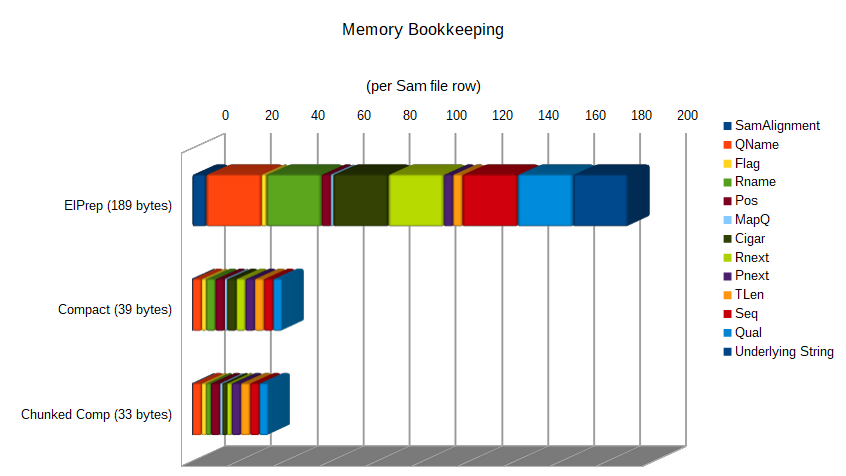
\includegraphics[scale=0.35]{images/MemoryBookeeping.png}
%\end{center}


%As this is a major reduction in memory consumption, let us analyze the techniques used to achieve this result.

The basic idea is that instead of storing an array of {\texttt{String}} objects, for example:
{\tt String items[] = \{"abc", "def"\}}, each consuming memory due to their headers, we can use 
a single object of type {\texttt{String}}, storing all the characters, and an additional array for their lengths.
\begin{verbatim}
String dataPool = "abcdef";
int[] endLengths = {3, 6};
\end{verbatim}

For such a small array, the save is minor, but for a large number of items (millions), the memory reduction becomes significant.
Even more important, the GC work is also reduced, since no matter how many items are in the {\texttt{dataPool}} and {\texttt{endLengths}} fields, there are only two objects to visit.
The technique described above was implemented in the class {\texttt{StringSequence}}.

If the strings that are to be stored are repeated frequently, we can apply another optimization:
instead of keeping them joined, we will use an indexed collection containing all the distinct strings and an array holding one index for each string.
For example, {\texttt{\{} "abc", "def", "abc", "xyz", "abc"\}} becomes:
\begin{verbatim}
table   : {abc=>0, def=>1, xyz=>2}
items   : [0, 1, 0, 2, 0]
\end{verbatim}
%The {\texttt{table}} structure is based on the class {\texttt{Object2IntOpenHashMap<String>}} from FastUtil library, instead of the standard {\texttt{HashMap<Integer, String>}}, since it uses the primitive data type {\texttt{int}} for representing the keys, which also saves some memory.
This data deduplication technique~\cite{he:2010},~\cite{manogar:2014} was implemented in the class {\texttt{DeduplicatedDictionary}}.

When storing strings containing characters from a restricted alphabet, one optimization that can be performed is using an array of primitive values, for example a {\texttt{long}[]}, and encoding each character into a block of bits.
The number of bits required for a character depends on the size of the alphabet.
DNA sequences use four letters {\texttt{A,C,G,T}}, but it is possible for a machine to read incorrectly a symbol and to return {\texttt{N}}.
In order to represent $5$ possible characters we need at least $3$ bits,
which as a result {\texttt{long}} can store in its $64$ bits $21$ DNA letters.
%The class {\texttt{DnaEncodingSequence}} which implements this string encoding technique contains the following members:
%\begin{verbatim}
%  LongArrayList content;
%  ShortArrayList lengths;      
%  IntArrayList positions;     
%\end{verbatim}
For example, encoding the $21$ letters string "AAAACCCCGGGGTTTTNNNNA" would produce a single long value, containing the bits (from right to left, $000$ represents A, $001$ represents C, and so on):\\
{\texttt{00001001001001000110110110110100
10010010001001001001000000000000}

}

In the sample files, one DNA sequence is typically around $100$ letters, so the memory needed in order to represent it would be $1$ {\texttt{int}} (encoding length) and $5$ {\texttt{long}}s (the content), that is $44$ bytes.
This reduces the memory consumption by a factor of two.

%Another advantage of using such an encoding is that when checking if two sequences are exactly the same, we can compare first their lengths and, if they are equal, comparing {\texttt{long}} values means comparing $21$ characters at once.
%As before, the GC will also benefit from the reduced number of objects that must be visited.


Running the smaller input file (144 MB), we have estimated that the original elPrep algorithm would use around three times more memory than the size of the input SAM file.
However, when trying to process the larger input file (1.2 GB), on a 32 GB machine, we have obtained an {\texttt{OutOfMemoryError}}, meaning that the penalty of using too many objects in order to represent the information was preventing us in loading the entire data set into memory.


On top of this, there is the cost of tags. 
In order to address {\texttt{temps}} and {\texttt{TAGS}} we have implemented the {\texttt{TagSequence}} class, which is a combination between {\texttt{StringSequence}} and {\texttt{DeduplicatedDictionary}}.
Without detailing all the calculations, in the original implementation, for the smallest file (144 MB), containing $2.1$ million rows, the JVM will use almost one gigabyte ($1,001,700,000$ bytes) just for object bookkeeping.
Our model will use much less additional memory, a $10\times$ saving for object bookkeeping.
For $2.1$ million entries, the tags memory consumption is now $50,400,000$ bytes and the combined value for the whole model is $132,300,000$ bytes (about $126$ MB).
%The version using chunking and batching offers some extra savings, as it uses $6$ bytes less per row.
%The used memory is $(33 + 24) * 2.1$ million $= 119,700,000$ bytes, about $10\%$ less than the {\textit{Compact} } version.


%In the original implementation, every {\texttt{SamAlignment}} object has references to {\texttt{temps}} and {\texttt{TAGS}} arrays.
%These arrays have an initial size of $16$, respectively $4$, and contain references to {\texttt{Field}} objects, which in turn contain a reference to a {\texttt{Slice}} object.
%These $20$ references and the extra two \texttt{ArrayList} instances imply that there is an additional fixed overhead of $20$ (references) $*8$ bytes $+ 2$ (\texttt{ArrayList}) $* 64 = 288$ bytes which are on top of the original elPrep's row store memory usage.
%In our calculation, the row without tags is $189$ bytes and the tags/temp cost another $288$,
%that is $477$ bytes (rounded up to $480$ by the JVM).
%That means that for the smallest file (144 MB), containing $2.1$ million rows, the JVM will use almost one gigabyte ($1,001,700,000$ bytes) just for object bookkeeping.
%
%In order to address {\texttt{temps}} and {\texttt{TAGS}} we have implemented the {\texttt{TagSequence}} class, which is a combination between {\texttt{StringSequence}} and {\texttt{DeduplicatedDictionary}}.
%Since the {\texttt{tags}} are repeating frequently, we save them using one {\texttt{short}} value per tag, but instead of using a list of tags, we define a sequence of indices.
%\texttt{TagSequence} does memory compaction by using a mix of \texttt{short} per-tag encoding and a joining the full sequence of tags.
%
%For example, for the input {\texttt{"tag0 tag1 tag2", "tag1 tag2 tag3"}}, the representation would be:
%\begin{verbatim}
%table = {"tag0":0, "tag1":1, 
%         "tag2":2, "tag3":3},
%lengths: [0,3], 
%tagSequence = [0,1,2,1,2,3]; 
%\end{verbatim}
%
%Our model will use much less additional memory: $4$ bytes for \texttt{lengths}, and each index pointing to the \texttt{table} would require $2$ bytes. On average, there are $10$ tags per row, so object bookkeeping would cost an extra $4 + 2*10 = 24$ bytes per row, a $10\times$ saving.
%
%For $2.1$ million entries, the tags memory consumption is now $50,400,000$ bytes and the combined value for the whole model is $132,300,000$ bytes (about $126$ MB).
%The version using chunking and batching offers some extra savings, as it uses $6$ bytes less per row.
%The used memory is $(33 + 24) * 2.1$ million $= 119,700,000$ bytes, about $10\%$ less than the {\textit{Compact} } version.


\section{\uppercase{Optimizing I/O Operations}}
\label{sec:io}

\subsection{\uppercase{Buffering and Synchronization}}
\label{subsec:buffering}

The elPrep algorithm starts by reading the input file. 
Based on the read information, it creates a large data set in memory and, in the end, it writes the processed data into another file.
In the writing step, the algorithm creates parallel tasks, which in turn take all \texttt{SamAlignment} instances and serialize them into the string format of SAM files.
Especially when the full data set is loaded into memory, these tasks create many small objects that have a negative impact in terms of memory management. Using a simple technique of {\textit{pre-allocating} } the buffer sizes based on the specific context of the problem, we can prevent the creation of many of these intermediate objects.

The code sequence that captures the writing process is presented below:
\begin{verbatim}
var outputStream = alnStream
  .parallel()
  .map((aln) -> {
    var sw = new StringWriter();
    try (var swout = new PrintWriter(sw))
      { aln.format(swout); }
    return sw.toString();
});
\end{verbatim}

An important technique that could improve performance when working with data is {\texttt{buffering}} \cite{oaks:2014}.
If we take a closer look at the {\texttt{StringWriter}} class we notice that it uses an internal {\texttt{StringBuffer}} object for storing its data, which in turn has an internal primitve buffer   which has $16$ characters as default.
The average length of a row in the input file is $325 - 330$ characters.
As $350$ is about $10\%$ larger than the average line, based on the regular statistical distribution, thus most lines would require no extra resizes of their corresponding buffers. This prevents the creation of extra garbage, which in turn reduces the number of times when GC is executed.
%So, the previous line would look like this: {\tt var sw = new StringWriter(350);}
In the following sections, we will denote the algorithm that employs this technique as {\textit{PresizedBuffers} }.


We will further analyze the usage of the \texttt{StringWriter} and its \texttt{StringBuffer} helper.
To quote from its documentation, a {\texttt{StringBuffer}} is  a thread-safe, mutable sequence of characters.
Meaning that most of its methods are declared as {\textit{synchronized}} in order to control the access to the buffer of characters in a multi-threaded environment.
However, in our case, each writing thread spawned by the parallel stream implementation gets its own copy of a {\texttt{StringWriter}} so there is no resource contention that would require synchronization.
Instead of using a {\texttt{StringWriter}}, it would be better to simply use a common buffer, with no synchronization.
Instead of creating and storing individual string representations of all the {\texttt{SamAlignment}} objects, and writing them one by one to disk, we add progressively information into the buffer.
Only when the buffer becomes full, we write its content on disk.
Obviously, all these steps will be performed in a single thread, but the bottleneck will be less obvious.
The class implementing the byte array is called {\texttt{StreamByteWriter}}.




%The most important technique that could improve performance when working with large files is I/O {\texttt{buffering} } \cite{oaks:2014}.
%%Invoking a Java {\textit{read} } method, for example, will eventually trigger an invocation to the operating system method responsible with reading data from the disk.
%%Although most operating systems use I/O buffering by default, an invocation of a method outside JVM is nevertheless expensive. Another reason to minimize the number of I/O operations is that, for each one of them, temporary objects needed to store the data must be created, meaning that GC will have more work to do when recovering the memory. 
%
%
%The elPrep algorithm starts by reading the input file. 
%Based on the read information, it creates a large data set in memory and, in the end, it writes the processed data into another file.
%In the writing step, the algorithm creates parallel tasks, which in turn take all \texttt{SamAlignment} instances and serialize them into the string format of SAM files.
%Especially when the full data set is loaded into memory, these tasks create many small objects that have a negative impact in terms of memory management. Using a simple technique of {\textit{pre-allocating} } the buffer sizes based on the specific context of the problem, we can prevent the creation of many of these intermediate objects.
%
%The code sequence that captures the writing process is presented below:
%\begin{verbatim}
%var outputStream = alnStream
%  .parallel()
%  .map((aln) -> {
%    var sw = new StringWriter();
%    try (var swout = new PrintWriter(sw))
%      { aln.format(swout); }
%    return sw.toString();
%});
%\end{verbatim}
%
%If we take a closer look at the {\texttt{StringWriter}} class we notice that it uses an internal {\texttt{StringBuffer}} object for storing its data, which in turn has an internal primitve buffer.
%This buffer has an initial capacity and it is resized whenever the text that must be represented no longer fits into it. When the buffer is full, its capacity is doubled. 
%The default size of a \texttt{StringBuffer} is $16$ characters, so creating a text of length $400$ would require $5$ resize operations, from $16$ to $512$. 
%
%The average length of a row in the input file is $325 - 330$ characters.
%As $350$ is about $10\%$ larger than the average line, based on the regular statistical distribution, this means that most lines would require no extra resizes of their corresponding buffers. This prevents the creation of extra garbage, which in turn reduces the number of times when GC is executed.
%
%So, by simply {\textit{pre-sizing} } the internal buffer of the \texttt{StringWriter} with the initial capacity of $350$ we could obtain note-worthy memory and runtime savings:
%{\tt var sw = new StringWriter(350)}.
%
%In the following sections, we will denote the algorithm that employs this technique as {\textit{PresizedBuffers} }.



%\subsection{\uppercase{Synchronization}}
%\label{subsec:sync}
%
%We will further analyze the usage of the \texttt{StringWriter} and its \texttt{StringBuffer} helper.
%To quote from its documentation, a {\texttt{StringBuffer}} is  a thread-safe, mutable sequence of characters.
%That means that most of its methods are declared as {\textit{synchronized}} in order to control the access to the buffer of characters in a multithreaded environment.
%However, in our case, each writing thread spawned by the parallel stream implementation gets its own copy of a {\texttt{StringWriter}} so there is no resource contention that would require synchronization.
%Instead of using a {\texttt{StringWriter}}, it would be better to simply use a common buffer, with no synchronization.
%To maximize the performance gain, the buffer could be implemented as a byte array.
%Using bytes instead of characters is quite trivial as Java {\texttt{String}} class has the method {\texttt{getBytes}()} and recreating a {\texttt{String}} object can be done by simply using one of its constructors: {\texttt{new String(bytes)}}.
%
%Writing to the file is implemented by simply invoking the {\texttt{println}} method of a {\texttt{PrintWriter}} output stream, decorating a {\texttt{BufferedWriter}}, which in turns decorates a {\texttt{FileWriter}}.
%\begin{verbatim}
%var out = new PrintWriter(
%  new BufferedWriter(
%    new OutputStreamWriter(output)));
%...    
%outputStream.forEachOrdered(
%  (s) -> out.println(s));
%\end{verbatim}
%
%Again, the {\texttt{PrintWriter.println}} method is using a {\texttt{synchronized}} block in order to fulfill its task, which is eventually an invocation to {\texttt{BufferedWriter.write}} method.
%\begin{verbatim}
%public void println(String x) {
%  synchronized (lock) {
%    print(x); println();
%   }
%}
%\end{verbatim}
%The {\texttt{BuffereWriter.write}} method is also synchronized and so is {\texttt{FileWriter.write}}, which is the last one invoked in this chain.
%
%Since more than half of the I/O time is spent writing, we have analyzed the CPU utilization, using the operating system profiler.
%
%%\begin{center}
%%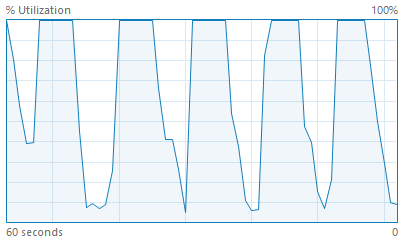
\includegraphics[scale=0.5]{images/cpu_original.png}
%%\end{center}
%
%The graph looks like a chainsaw, which is a sign that the code is bottle-necked on a single thread.
%This is no surprise, since the {\texttt{outputStream}} is written in a sequential fashion.
%On top of that, for every row there has to be a mutex check whenever a synchronized block of code is invoked.
%Since there are a large number of rows, all these checks will add up and produce a significant slowdown of the overall writing process.
%
%The technique that should have been used in this context involves using a single byte array.
%Instead of creating and storing individual string representations of all the {\texttt{SamAlignment}} objects, and writing them one by one to disk, we add progressively information into the buffer.
%Only when the buffer becomes full, we write its content on disk.
%Obviously, all these steps will be performed in a single thread, but the bottleneck will be less obvious.
%The class implementing the byte array is called {\texttt{StreamByteWriter}}.
%\begin{verbatim}
%StreamByteWriter streamByteWriter 
%  = new StreamByteWriter(output);
%for (SamAlignment aln: alignments) {
%  aln.formatBuffer(streamByteWriter);
%}
%\end{verbatim}
%Even if we are using now a single core for all the writing, the necessary time for creating the output file was reduced by half.
%
%%The following graph shows the CPU utilization for this approach:
%%\begin{center}
%%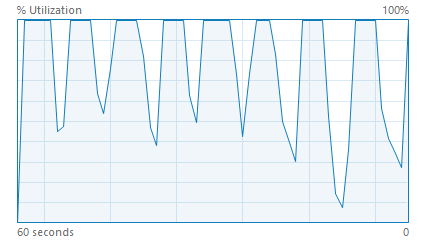
\includegraphics[scale=0.5]{images/cpu_optimized.png}
%%\end{center}
%
%In the previous graph, capturing the repeated execution of the algorithm, it is still visible that the CPU jumps from using all cores, when reading, to using only one core, when writing, however the idle time is reduced and this ensures a significant reduction in the running time.


\subsection{\uppercase{Chunking-Batching and Extracting Parallelism}} 
\label{subsec:batching}

In the elPrep original algorithm, a {\texttt{SamAlignment}} object is created for each row in the input file.
In order to extract parallelism, there is an explicit {\texttt{.parallel}()} call, a construct that would create a task for each row that must be processed.
These tasks are queued and executed in a concurrent fashion using threads created transparently by the Java Stream API.
\begin{verbatim}
var alnStream = inputStream.parallel()
  .map((s) -> new SamAlignment(s));
\end{verbatim}
In the column-based model, described in section~\ref{subsec:column}, there is a single {\texttt{SamBatch}} instance storing all the data.
Because we perform data compaction, the {\textit{read}} operation must take into account the dependencies between rows.
Just like in the case of removing duplicates, in order to process a new row we have to inspect the values of the previously read rows.
Therefore the reading process cannot be fully parallel per-row.
In order to obtain a better performance than reading using a single thread, we propose a technique that splits the {\texttt{SamBatch}} structure in several "chunks".
Instead of having a single large object, we will represent the data using an array of smaller {\texttt{SamBatch}} objects.
A sketch of our {\textit{Compact}} algorithm is described by the following pseudo code:

\begin{verbatim}
int chunkSize = 20000;
int nbOfThreads = cpuCoreCount * 4;
var samBatches = new ArrayList<SamBatch>();
while (!endOfFile) {
  var rowsRead = parallelReadRows(
    batchSize, nbOfThreads);
  parallelTransformRowsIntoBatches(
    samBatches, rowsRead);
}
\end{verbatim}

The {\texttt{readRows}} method reads $chunkSize * nbOfThreads$ rows out of the SAM file for the next processing step.
The actual reading is done using an appropriate number of threads (based on the CPU configuration), each thread reading sequentially a fixed number of rows, calculated taking into account the nature of the information being encoded.
Having the data split into chunks, we can process in parallel the mapping between the associated text and the {\texttt{SamBatch}} data structure, where we perform data compaction and deduplication.
The techinque of grouping similar tasks requiring the same resources in order to streamline their completion is called {\textit{batching}}.

In our case, the advantages of the chunking-batching approach are multiple.
%Transforming data, deduplicating and DNA encoding are now all executed in a single-threaded manner, which is much easier to debug and understand than a multithreaded equivalent.
Since a {\texttt{DeduplicatedDictionary}} will now have less than $20000$ unique strings, the values needed to encode the strings could be represented on $2$ bytes, instead of $4$.
Similarly, we can reduce the tag size from $4$ to $2$ bytes.
After the algorithm is fully executed,  we will have instead of $2.1$ million {\texttt{SamAlignment}} objects, about $105$ {\texttt{SamBatch}} instances, each of them having around $4$ orders of magnitude less objects overall.
This translates into $2$ orders of magnitude less objects.
When creating the output file, the {\texttt{SamBatch}} array could be processed in parallel, with no blocking except the actual operation of writing to disk.

We have seen that the column-based model saves memory at the expense of the running time.
This optimization, however, reduces the overall execution time of the read operation, which is now on par with the original implementation.

When it comes to writing, compared to our {\textit{StreamByteWriter} } algorithm, which is anyway much faster than the original implementation, the execution time is drastically reduced from $28$ seconds (for the $12$ GB BAM file) to $12$ seconds.
Preparing the strings that are to be written in the file can be done in almost perfect parallelism, using the available cores.
The only limitation remains the speed of the output device, which can vary depending on its type: in-memory virtual partition, SSD, HD, etc.

In order to make sure there are no dead times when using the external device, 
we have also implemented the {\textit{async/await}} pattern.
This allows the program to perform in advance reading operations, using a dedicated thread, while waiting for the data processing threads to complete their execution.
This new algorithm, called {\textit{Compact/Par}}, offers a small improvement in the running time, as we will see in the next section, but with the disadvantage of a significant increase in code complexity.




\section{\uppercase{Experimental Results}}
\label{sec:results}

\subsection{\uppercase{Overview}}
\label{subsec:overview}

We have created five implementations that address the most expensive parts of the elPrep algorithm, which are reading,  storing all data in the memory and writing.
Except for the original version, which was taken from elPrep public repository, all other algorithm implementations contain various types of optimization that are meant to improve runtime performance and to lower the memory usage, especially on large files where GC becomes a limiting factor. 
%We recap the names of the algorithms as they are used in the following sections:
%\begin{itemize}
%\item {\textit{Original} }, the original algorithm described in~\cite{costanza:2019};
%
%\item {\textit{PresizedBuffers} } reduces the number of memory allocations by appropriate initialization of the data structures that hold the data to be written, taking into consideration the specific size of the file rows;
%
%\item {\textit{StreamByteArray} } transforms string into bytes and writes them directly into an \texttt{OutputStream}, reducing to almost zero the number of memory allocations related to writing.
%
%\item {\textit{Compact} } employs a more elaborate column-based model for storing the data set in a "compact" form, instead of the simple row-based approach used in the previous two algorithms; this reduces drastically the memory usage at the expense of running time.
%
%\item {\textit{Compact/Par} } represents a modified variant of the {\textit{Compact} } algorithm aimed at reducing to a minimum the dead times regarding I/O operations.
%
%\end{itemize}


The computer we have used in order to perform the experiments is a Ryzen 9-3900X, having 12 cores and using 48 GB of RAM\@.
Since we didn't have access to the hardware necessary to run all the tests in memory, as the original paper, we have used the smaller SAM files and ran the same processing repeatedly in order to obtain an accurate result of the running time.
For example, running $10$ times the algorithm on the smallest input SAM file, which is approximately $700$ MB, will produce a total running time of around $70$ seconds. 
Running the algorithm repeatedly will trigger the garbage collector and this will be the cause of variations in the collected results, ranging from around $2$ to $3$ seconds, when reading the smallest file, and $3$ to $4$ seconds for writing.

%Before executing the timed invocations, we have {\textit{warmed-up}} the JVM\@.
%This is usually achieved by simply running a couple of times an initial test (not timed) that uses all the classes involved in the algorithm.
%Such a warm-up is necessary because Java is using a lazy class loading mechanism and just-in-time compilation.
%After this step, all important classes are stored into the JVM cache (native code), making them available at runtime with no additional penalty.

The original elPrep benchmarks have been performed on a Supermicro SuperServer 1029U-TR4T node with two
Intel Xeon Gold 6126 processors consisting of 12 processor cores each, clocked at 2.6 GHz, with 384 GB RAM~\cite{costanza:2019}.
The authors claim to do the processing of the 8 GB BAM file in 6 min:54sec to 7 min:31sec and memory usage is $330-340$ GB\@.

As we didn't have access to such a performing machine, we did most of testing with the smallest file, the $144$ MB BAM file ($673.3$ MB SAM file). For the $8$ GB BAM file ($27.18$ GB SAM) our results will show only the {\textit{Compact} } algorithm but we will make some inferences over the scaling of the algorithms across file sizes and cores.

%Since the elPrep algorithm is designed to run everything in memory, we tuned the JVM heap size (using the \texttt{-Xmx} flag) to the maximum value allowed by the operating system. 

%In order to analyze the performance of read/write operations, we made sure that no background OS services are running during our tests, by manually stopping them.



\subsection{\uppercase{Runtime performance}}
\label{subsec:runtimeperf}

The following table shows a brief comparison of the running times obtained by our algorithms, in three configurations: $144$ MB file using $4$ cores and $12$ cores, and $1.2$ GB file using $12$ cores. 

\begin{small}
\begin{center}
\textbf{Running time per algorithm in seconds} \\
\begin{tabular}{|C{2cm}|C{1.2cm}|C{1.2cm}|C{1.2cm}|}
\hline
						& 144 MB (4c)	& 144 MB (12c)		& 1.2 GB (12c)	\\ \hline
Original				& 9.13 			& 3.938 			& 123.91 		\\ \hline
PresizedBuffers			& 8.98 			& 4.19 				& 75.1 			\\ \hline
StreamByteArray			& 8.09 			& 3.43 				& 64.62 		\\ \hline
Compact 				& 5.64 			& 3.4 	 			& 34.5			\\ \hline
Compact/Par 			& 5.42		    & 4.68				& 26.7 			\\ \hline
\end{tabular}
\end{center}
\end{small}

%The largest file shows the following numbers:
\begin{center}
	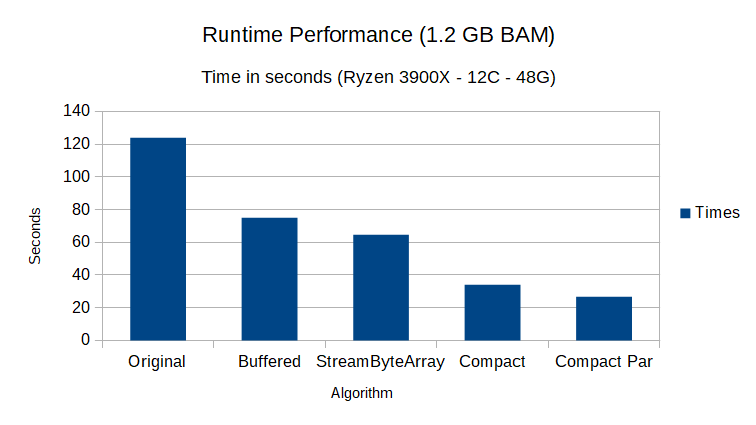
\includegraphics[scale=0.5]{images/runtime_perf_1_2G.png}
\end{center}

Comparing $4$ cores to $12$ cores, we notice that the {\textit{Original} } algorithm scales with a factor of $2.3$, {\textit{PresizedBuffers} } by a factor of $2.14$, {\textit{StreamByteArray} } scales by $2.36$ and {\textit{Compact} } would scale by $1.69$. So, at least for the small file, it seems that using larger machines will offer a better performance. It is important to notice that, in its current implementation, the {\textit{Compact} } algorithm has an explicit sequential part that reduces its scalability.
Some potential fixes are described in section \ref{sec:future}, where we describe some techniques aimed at improving the single threaded part.

A more useful way to present the algorithm is to show how it scales based on input size, and at least on the 12 core machine, we can see that both compact algorithms remain roughly in the same speed, so GC's runtime cost doesn't become in impediment:

\begin{center}
	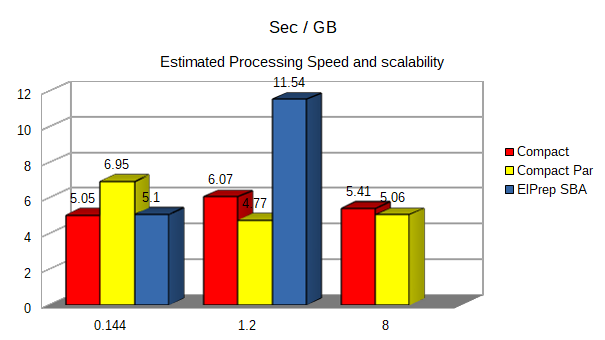
\includegraphics[scale=0.5]{images/seconds_per_gb_ryzen.png}
\end{center}

%Comparing $4$ cores to $12$ cores, we notice that the {\textit{Original} } algorithm scales with a factor of $2.3$, {\textit{PresizedBuffers} } by a factor of $2.14$, {\textit{StreamByteArray} } scales by $2.36$ and {\textit{Compact} } would scale by $1.69$. So, at least for the small file, it seems that using larger machines will offer a better performance. It is important to notice that, in its current implementation, the {\textit{Compact} } algorithm has an explicit sequential part that reduces its scalability.
%Some potential fixes are described in section \ref{sec:future}, where we present some techniques aimed at improving the single-threaded part.
%
%Considering the file size, the elPrep algorithm uses a lot of memory and, since the JVM has to call more often the Garbage Collector, the cost of GC visibly influences the executing time, affecting its scalability. Our techniques of reducing object allocations presented in {\textit{PresizedBuffers} } and {\textit{StreamByteArray} } algorithms pay off now, their runtime profiles being much better than the original. Since the {\textit{Compact} } algorithm reduces drastically the memory consumption, it is not affected too much by GC and the overall running time is significantly superior.
%For an increase in file size $8$ times, the {\textit{Original} } algorithm would slow down $31.46$ times, the {\textit{PresizedBuffers} } will slow down $17.92$ times, {\textit{StreamByteArray} } will slow down $18.83$ times,
%and the {\textit{Compact}} algorithm will have an almost perfect $8.33$ times slow down.
%
%For the $8$ GB BAM file, we could only execute the {\textit{Compact} } algorithm, as the others elPrep derived algorithms would produce an \texttt{OutOfMemoryError}, even when setting the heap size up-to $42$ GB.
%The execution time was around $215$ seconds, so as we are reaching the limits of the machine, for a file that is approximately $5$ times larger, the algorithm slows down by a factor of $12$. When moving the input file to an SSD, which offers a faster I/O, the running time drops to $139.8$ seconds, which means a $10$ times slow down.



\subsection{\uppercase{Memory Usage}}
\label{subsec:memusage}
To measure the live data set, we have used Java VisualVM \cite{visualvm:oracle} which provides a visual interface for profiling a running application. Using VisualVM, we have analyzed the memory consumption in each scenario and we have estimated the minimum amount of memory that JVM requires in order to load a specific data set.

Unlike the original paper, which measures process memory size, we have measured live data size.
This is possible due to VisualVM which offers very precise information regarding the objects consuming memory.

%It is also important to understand that the more live memory is used, and more complex the graph of objects is and the less free memory exists on a particular machine, the GC impact will be higher.
%This is because the GC algorithm is triggered when a critical amount of the heap is occupied.
%Therefore, the more memory JVM has access to, the more seldom GC will execute.
%The default {\textit{Garbage First Garbage Collector}  (G1 GC)} is automatically triggered at $45\%$ memory occupancy (this value being configurable using the \texttt{InitiatingHeapOccupancyPercent} parameter). When the heap is reaching this level, JVM will spawn background threads in order to do the marking phase, and this affects the running time.
%Having a larger machine with double memory will trigger the GC at least two times more seldom and
%although the number of objects to be removed is the same, the overall time necessary for this operation is improved.

\begin{small}
\begin{center}
\textbf{Memory usage per algorithm in MB} \\
	\begin{tabular}{|c|c|c|}
		\hline			  	& 144 MB file		& 1.2 GB file		\\ \hline
		Original			& 2326 MB			& 32025 MB			\\ \hline
		PreSizedBuffers		& 2326 MB			& 32025 MB			\\ \hline
		StreamByteArray 	& 2275 MB			& 31463 MB			\\ \hline
		Compact/Par			& 606 MB			& 4689 MB			\\ \hline
	\end{tabular}
\end{center}
\end{small}

\begin{center}
	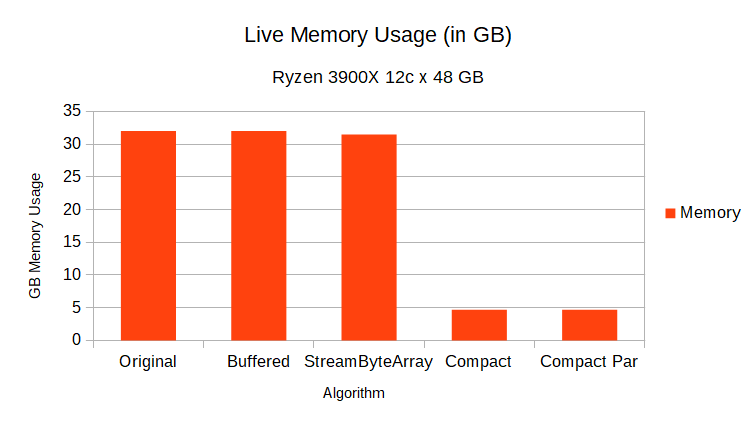
\includegraphics[scale=0.5]{images/memory_usage_1_2G.png}
\end{center}

The peak usage was measured by suspending the program at the moment when the whole file was read.
We notice that for the $1.2$ GB BAM file, the {\textit{Original} } and {\textit{Presized Buffers} } algorithms are using around $32$ GB of memory. In order to offer this amount of memory to JVM we used a machine with $48$ GB of RAM. To further reduce the overhead of GC, $64$ GB would certainly have been better.

%On a $48$ GB machine, {\textit{Compact} } algorithms can process larger files: the $8$ GB BAM file uses $24283$ MB of live data and the $12$ GB BAM input uses $35 265$ MB.


%We also have to note that not all of the used memory represents data related to the input file.
%For example, in the case of the original elPrep algorithm, as it creates millions of tasks even for the smallest $144$ MB BAM file, Java Streams library will create a queue of objects that will remain in memory very likely until the end. This might add maybe around $100$ MB of memory, as it is quite hard (if not impossible) to measure it.

 
 
\subsection{\uppercase{Calculating Performance}}
\label{subsec:performance}
The goal of elPrep was to keep both the running time and the the memory consumption low. The evaluation function was defined as the multiplication of the average elapsed wall-clock time (in hours) with the average maximum memory use (in GB), with lower values (in GBh) being better \cite{costanza:2019}.
We have used the same approach, changing only the measurement units to MB and seconds.


%In order to analyze the impact of the hardware to the performance of the algorithms, we have executed the tests on two distinct machines: the Ryzem 3900X ($1$2 cores and $48$ GB RAM) and a laptop with $4$ cores and $16$ GB RAM.

%The results for the $144$ MB file are presented below (lower bars are better):
%\begin{center}
%	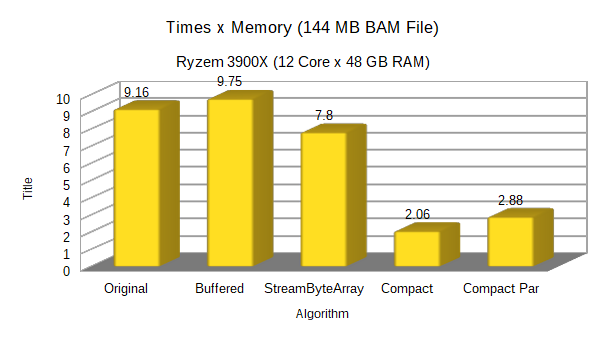
\includegraphics[scale=0.5]{images/times_and_memory_chart_small_144mb_ryzen.png}
%\end{center}

%As the memory usage is quite similar between the \textit{Original}, \textit{PresizedBuffers} and \textit{StreamByteArray} algorithms, their comparative performance is influenced only by the runtime savings.
%Both \textit{Compact} algorithms are on par from the point of view of the running time, but since they are using far less memory their performance is much better.
%
%We observe that the combination of small size of the file (meaning the algorithm will run just in seconds) and the high core count (12 cores) has a negative impact on the more elaborate algorithm \textit{Compact/Par} which has a small slow-down compared to the more simple \textit{Compact} implementation.
%
%On the laptop (which has a better SSD), the {\textit{Compact} } algorithm performs even better, since it could not fully exploit the high number of cores in the first test:

%\begin{center}
%	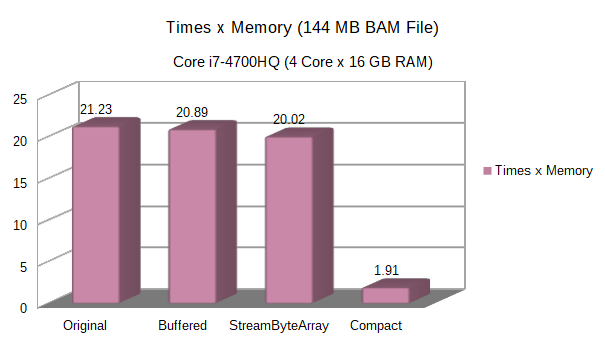
\includegraphics[scale=0.5]{images/times_and_memory_chart_small_144mb_intel.png}
%\end{center}

On the medium file ($1.2$ GB BAM) the values are conclusive from the point of view of scaling the results. The improvements resulting from our optimization techniques are now clearly visible.
\begin{center}
	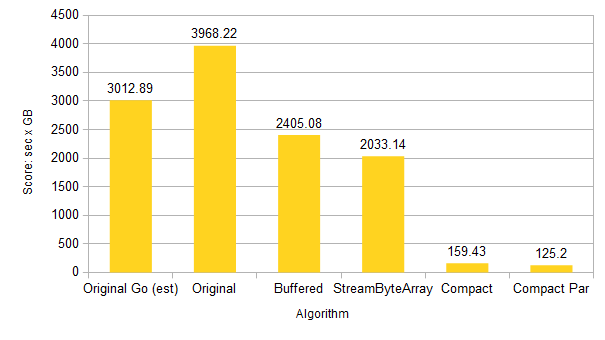
\includegraphics[scale=0.5]{images/times_and_memory_chart.png}
\end{center}



%For the larger files, since we could only run the \textit{Compact} and \textit{Compact/Par} algorithms, we can't make a direct comparison between all algorithms. To overcome this impediment, we have calculated estimated values based on the scaling factors obtained from the files we could run.
%We compared the \textit{StreamByteArray} algorithm, which should scale better than the \textit{Original}, to the \textit{Compact} versions, calculating the number of GBs processed per second.
%
%The average values, including both read and write operations, are presented below:

%\begin{center}
%	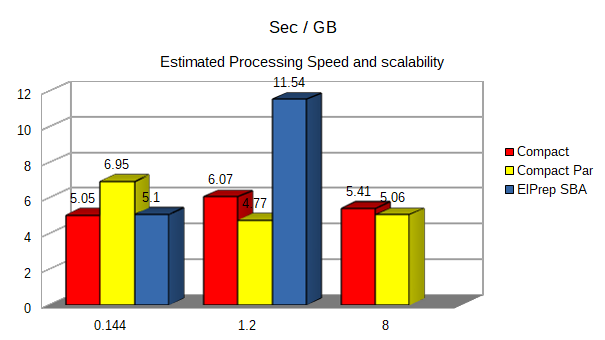
\includegraphics[scale=0.5]{images/seconds_per_gb_ryzen.png}
%\end{center}

Tests performed up-to the $8$ GB file showed that algorithms scale as expected, GC does not become a large impediment for the \textit{Compact} implementations and the overall performance seems limited only by other hardware components, such as disk drive read/write speeds.
Both \textit{Compact} algorithms keep a steady pace of processing at around $180$ MB/second (under $6$ seconds to process every $1$ GB of BAM). \textit{StreamByteArray} has a sharp loss of speed as GC is triggered more often, processing data at half speed when increasing the BAM file size from $0.144$ GB to $1.2$ GB.









\section{\uppercase{Future work}}
\label{sec:future}

\textbf{Batch reader scalability} \\
As we have described in section \ref{subsec:batching}, our {\textit{batch reader} } works in two steps: initially, on the main thread, it extracts from the original file the rows for the number of the expected batches, and then it executes in parallel, using all cores, the data compaction step.
Before chunking and batching is done, we split the full byte array read from file into distinct  \texttt{List<byte[]>} instances.
This separation may not be necessary, an alternate approach being to store inside a large \texttt{byte[]} structure all the information and to use an additional array of indices in order to retrieve the actual lines of text.
This would reduce the number of allocations and eventually speed up the execution of the main thread.

%A similar variation of speeding up the single threaded part is to not do the line splitting at all, but to read a block of text in advance, that would be around the expected chunk size,
%and then split it in lines in a multithreaded way.

\textbf{Value Types} \\
When Java specifications were elaborated, more than $25$ years ago, the cost of a retrieving an object from the memory and executing an arithmetic operation was approximately the same.
On modern hardware however, the memory fetch operations are up to $1000$ times more expensive than arithmetic ones.
This is why, the {\textit{Project Valhalla} } \cite{jdk:valhalla}, that is expected to be integrated in modern JDK releases, introduces new data structures and language constructs that improve various aspects regarding data manipulation.
For example, {\textit{Value Types} } provide the necessary infrastructure for working with immutable and reference-free objects.
In our context, this would allow us to further reduce the memory used by the {\textit{Compact} } algorithm by using an efficient by-value computation with non-primitive types.



\section{\uppercase{Conclusions}}
\label{sec:conclusions}
This paper addresses the situation when one has to manipulate a large textual data set by reading it from a file, transforming it into objects, processing it and then writing it back to a file, and all these operations must be performed in a single in-memory session.
We have analyzed a modern implementation of an algorithm for processing SAM and BAM files, elPrep \cite{herzeel:2015}, \cite{herzeel:2019}, which must handle input files up to $100$ GB.
The conclusion of the elPrep authors was that a Java implementation for this specific problem suffers from the memory management offered by JVM \cite{costanza:2019}.
However, when using an object-oriented programming platform, one has to take into consideration all aspects regarding memory allocation offered by that specific platform and to adapt its model and programming techniques.
%Since Java is a general purpose programming platform, it offers a standard set of classes and language constructs providing a balance between performance and ease of use.
%When dealing with hard problems, one has to analyze the default behavior of the programming interface and "tweak" it accordingly.

We have showed that major improvements can be obtained by using techniques that are aimed at reducing the number of created objects.
This will not only save memory but it will also improve runtime performance by decreasing the overhead of the Garbage Collector.
Using a column-based representation we have compacted the data set in a manner that boosted the overall score calculated as the multiplication between used memory and running time.
The penalty incurred by the more elaborate data model was compensated by a multi-threaded approach, called chunking-batching, that actually allows the algorithm to use all available machine cores when processing the input file.
%In order to optimize the usage of the I/O device, we have implemented the {\textit{async/await} } pattern, which also offered a small increase in performance.

Given the hardware differences between the machine used by the elPrep authors and ours, there are limits on the testing that could be done with the techniques used by this paper.
%Instead of a $384$ GB of memory, dual-CPU server, we have used a machine  with $8$ times less RAM, half of CPU cores, a much slower disk drive (the SSD on the Ryzen machine can barely read at 300 MB/s, while a NVMe SSD can reach $32$ GB/s) and so on.
However, using input files ranging in size from $144$ MB to $12$ GB, we have proved that our algorithms are scalable and could perform as expected for files of any size, provided the machine has sufficient memory.





\bibliographystyle{apalike}
{\small
\bibliography{elprep-study}}


\end{document}

